\chapter{Đọc thêm 2: Dự đoán Thị trường Tài chính bằng Google Trends (Challet \& Bel)}
\label{ch:M4L2DT2}

% Nguồn: Challet, D., & Bel, A. ``Predicting financial markets with Google Trends and not so random keywords.'' arXiv, 2014.
% Phần cần đọc: Toàn bộ bài báo
% Nội dung bắt buộc đọc: được kiểm tra trong mọi bài đánh giá (kể cả Quiz).

\section{Thông tin nguồn}

\begin{itemize}
  \item \textbf{Nguồn:} Challet, Damien, and Ahmed Bel Hadj Ayed. \emph{Predicting financial markets with Google Trends and not so random keywords}. arXiv, 2014. \url{https://doi.org/10.48550/arXiv.1307.4643}
  \item \textbf{Phần cần đọc:} Toàn bộ nội dung
\end{itemize}

\bigskip

\noindent\textit{Tác giả: Damien Challet (Chaire de finance quantitative, Laboratoire de mathématiques appliquées aux systèmes, École Centrale Paris, Grande Voie des Vignes, 92295 Châtenay-Malabry, Pháp; và Encelade Capital SA, Parc Scientifique C, EPFL, 1015 Lausanne, Thụy Sĩ) và Ahmed Bel Hadj Ayed (cùng chi nhánh École Centrale Paris nêu trên).}

\section{Tóm tắt}

Chúng tôi thảo luận về những tuyên bố cho rằng dữ liệu từ Google Trends chứa đủ thông tin để dự đoán lợi suất chỉ số tài chính trong tương lai. Trước tiên, chúng tôi rà soát nhiều sai lệch tinh vi (và ít tinh vi hơn) có thể ảnh hưởng đến việc kiểm định lùi (backtest) một chiến lược giao dịch, đặc biệt khi chiến lược đó dựa trên loại dữ liệu này. Như dự đoán, việc lựa chọn từ khóa đóng vai trò then chốt: bằng cách sử dụng một hệ thống backtest đạt chuẩn công nghiệp, chúng tôi xác nhận rằng các từ khóa ngẫu nhiên liên quan đến tài chính không chứa nhiều thông tin dự đoán có thể khai thác hơn so với các từ khóa ngẫu nhiên liên quan đến bệnh tật, xe cổ và trò chơi thùng (arcade games). Tuy nhiên, các từ khóa khác khi áp dụng lên những tài sản phù hợp lại tạo ra các chiến lược giao dịch có lợi nhuận ổn định, qua đó xác nhận trực giác (intuition) của tài liệu tham khảo [24].

\section{I. Giới thiệu}

Việc đo lường nhịp đập của xã hội với tần suất và độ chính xác chưa từng có đang trở nên khả thi nhờ dữ liệu từ nhiều trang web khác nhau. Cụ thể, dữ liệu từ Google Trends (viết tắt là GT trong bài này) báo cáo mức độ quan tâm tìm kiếm (search volume interest, SVI) trong lịch sử đối với các từ khóa cho trước và đã được dùng để dự đoán hiện tại [7] (được gọi là \emph{nowcasting} trong [5]), nghĩa là để cải thiện ước tính các đại lượng đang hình thành nhưng số liệu của chúng chỉ được công bố vào cuối một giai đoạn nhất định. Các đại lượng này bao gồm số liệu thất nghiệp, du lịch và niềm tin tiêu dùng [7], lợi nhuận hàng quý của doanh nghiệp (từ các lượt tìm kiếm về sản phẩm chủ lực của họ) [8], ước tính Tổng sản phẩm quốc nội (GDP) [5] và dịch cúm [15].

Các nhà giao dịch xác định giá tài sản. Một số nhà giao dịch tìm kiếm, chia sẻ và cuối cùng tạo ra thông tin trên nhiều trang web khác nhau. Do đó, giá tài sản lẽ ra phải liên quan đến hành vi của người dùng website. Phép tam đoạn luận này đã được nghiên cứu chi tiết trong [9]: lợi suất giá của các cổ phiếu thành phần trong chỉ số Russell 3000 được hồi quy theo nhiều nhân tố, bao gồm dữ liệu GT, và các nhân tố này được lấy trung bình trên toàn bộ 3000 tài sản. Trong số các phát hiện khác, các tác giả nhận thấy một mối tương quan đáng kể giữa những thay đổi trong SVI và hoạt động giao dịch của nhà đầu tư cá nhân. Ngoài ra, tính trung bình, các biến động của SVI có tương quan âm với lợi suất giá trong khoảng vài tuần trong giai đoạn được nghiên cứu (tức là trong mẫu, in-sample). Nhu cầu lấy trung bình trên nhiều cổ phiếu xuất phát từ lượng nhiễu trong cả lợi suất giá lẫn dữ liệu GT, và từ việc chỉ một phần nhỏ những người tìm kiếm một từ khóa cho trước thực sự giao dịch sau đó.

Tuyên bố của [24] mạnh mẽ hơn nhiều: bài báo cho rằng lợi suất tương lai của chỉ số Dow Jones Industrial Average có tương quan âm với các bất ngờ SVI (SVI surprise) liên quan đến một số từ khóa nhất định, do đó dữ liệu GT chứa đủ thông tin để dự đoán các chỉ số tài chính. Một số sai lệch tinh vi (và không quá tinh vi) khiến kết luận của họ không thể mạnh mẽ như đáng lẽ phải có. Bằng cách sử dụng một hệ thống backtest chặt chẽ, chúng tôi có thể xác nhận rằng dữ liệu GT có thể được dùng để dự đoán lợi suất giá tài sản trong tương lai, qua đó đặt kết luận của họ trên một nền tảng vững chắc hơn nhiều.

\section{II. Dữ liệu và Chiến lược}

Giá tài sản thô được mô tả khá tốt bởi các bước đi ngẫu nhiên (random walk) phù hợp, vốn hoàn toàn không chứa khả năng dự đoán. Tuy nhiên, giá tài sản có thể trở nên dự đoán được nếu người ta có thể xác định một tập hợp điều kiện, sử dụng hoặc chỉ lợi suất tài sản (xem ví dụ [21] về các điều kiện dựa trên tương quan chéo giữa các tài sản) hoặc các nguồn thông tin bên ngoài. Google Trends cung cấp các chuỗi thời gian đã chuẩn hóa về số lượt tìm kiếm cho các từ khóa cho trước với độ phân giải thời gian theo tuần [28], ký hiệu là $v_t$. [24] đề xuất chiến lược giao dịch sau: định nghĩa mức độ quan tâm tìm kiếm cơ sở (baseline) trước đó là
$$
\bar v_t = \frac{1}{T}\sum_{t'=t-T}^{t} v_{t'},
$$
bất ngờ SVI (SVI surprise) là $\delta_t = v_t - \bar v_{t-1}$, và vị thế cần nắm giữ trên tài sản liên quan trong tuần $t+1$ là $s_{t+1} = -\text{sign}\,\delta_t$. Không có gì ngăn cản việc xem xét chiến lược nghịch đảo, nhưng hiện tượng đảo chiều giá trung bình (price reversion) trong một hoặc hai tuần tiếp theo tương ứng với một thay đổi của SVI đã được các tác giả khác ghi nhận trước đó [9, 11].

Thay vì cố gắng dự đoán chỉ số Dow Jones Industrial Average, chúng tôi sử dụng chuỗi thời gian của SPY, vốn phản ánh chỉ số Standard and Poor's 500. Điều này cung cấp một hình thức kiểm định chéo (cross-validation) yếu, vì hai chuỗi thời gian này có tương quan cao nhưng không hoàn toàn đồng nhất. Vì cùng lý do đó, chúng tôi tính lợi suất từ giá đóng cửa thứ Hai đến giá đóng cửa thứ Sáu thay vì từ thứ Hai đến thứ Hai, giúp giữ cho lợi suất chỉ số đồng bộ với dữ liệu GT (dữ liệu này trải dài từ Chủ nhật đến thứ Bảy).

\section{III. Các Sai lệch Phương pháp luận}

Dự đoán vốn đã khó, đặc biệt là dự đoán về tương lai. Nhưng dự đoán về tương lai trong quá khứ còn khó hơn. Điều này đặc biệt đúng với việc backtest một chiến lược giao dịch, tức là việc tính toán lợi nhuận ảo (virtual gains) của chiến lược đó trong quá khứ. Backtest dễ mắc phải nhiều loại sai lệch có thể làm thay đổi đáng kể độ tin cậy của nó, thường theo hướng tích cực (lạc quan hóa kết quả) [14, 20]. Phần lớn các sai lệch này bắt nguồn từ xu hướng đáng tiếc và có lẽ khó tránh khỏi của việc thông tin tương lai len lỏi vào quá khứ.

\subsection*{A. Sai lệch do công cụ}

Đây là sai lệch dễ bị bỏ qua nhất. Nó giải thích một phần lý do vì sao hiệu suất backtest thường rất tốt trong những năm 1980 và 1990, nhưng kém ấn tượng hơn kể từ khoảng năm 2003, ngay cả khi đã tính đến các ước tính thực tế về tổng chi phí giao dịch. Việc tìm ra khả năng dự đoán trong dữ liệu cũ bằng công cụ hiện đại thực sự dễ dàng hơn mức đáng lẽ phải có. Hãy hình dung việc áp dụng các phương pháp tốn nhiều tài nguyên CPU hoặc bộ nhớ lên dữ liệu từ thời kỳ trước khi có máy tính. Định luật nổi tiếng nhất về sự gia tăng năng lực tính toán mang tên Gordon Moore, người nhận thấy rằng số lượng bóng bán dẫn tối ưu trong mạch tích hợp tăng theo hàm mũ theo thời gian (với chu kỳ tăng gấp đôi $\tau \simeq 2$ năm) [23]. Nhưng các khía cạnh quan trọng khác của tính toán cũng đã và đang cải thiện theo hàm mũ, chẳng hạn như lượng tính toán trên mỗi đơn vị năng lượng (định luật Koomey, $\tau \simeq 1.5$ năm [18]) hoặc giá lưu trữ (định luật Kryder, $\tau \simeq 2$ năm [19]). Đáng chú ý, những tiến bộ công nghệ này được phản chiếu qua sự tiến hóa của khung thời gian phản ứng tối thiểu (minimal reaction timescale) trong dữ liệu tài chính [16]. Thêm vào đó, khả năng gần đây có thể huy động và giải phóng gần như tức thì những nguồn lực điện toán đám mây khổng lồ lên các tập dữ liệu lớn đã thay đổi cách thức phân tích dữ liệu tài chính. Rất khó để tính đến sai lệch này. Với mục đích giáo dục, người ta có thể làm quen với năng lực máy tính trong quá khứ bằng các máy ảo như \texttt{qemu} [2], được tinh chỉnh để mô phỏng tốc độ và bộ nhớ của các máy tính sẵn có tại một thời điểm nhất định với một số tiền nhất định.

Loại sai lệch tương tự cũng mở rộng sang những tiến bộ trong tài liệu thống kê và học máy, và thậm chí cả cách người ta hiểu về động lực học thị trường: việc sử dụng một phương pháp cụ thể có khả năng cho kết quả tốt hơn trước khi phương pháp đó được công bố so với, chẳng hạn, một hoặc hai năm sau đó. Người ta có thể mở rộng lập luận này sang tính lịch sử của các phương pháp được kiểm định trên dữ liệu tài chính tại bất kỳ thời điểm nào, bởi vì chúng đi theo trào lưu (fashion). Dù sao đi nữa, đây là một khía cạnh của backtest xứng đáng được nghiên cứu một cách hệ thống hơn.

\subsection*{B. Sai lệch dữ liệu}

Dữ liệu bị sai lệch theo hai cách. Thứ nhất, khi backtest một chiến lược phụ thuộc vào các tín hiệu bên ngoài, trước tiên người ta phải tự hỏi liệu tín hiệu đó có thực sự sẵn có vào các thời điểm mà nó ghi nhận hay không. Dữ liệu GT không sẵn có một cách đáng tin cậy trước ngày 6 tháng 8 năm 2008, vì khi đó dữ liệu chỉ được cập nhật một cách ngẫu nhiên vài tháng một lần [27]. Các backtest tại những thời điểm trước đó chứa đựng một phần khoa học viễn tưởng không thể tránh khỏi, nhưng vẫn hữu ích để hiệu chỉnh (calibrate) các chiến lược.

Vấn đề thứ hai là dữ liệu bị điều chỉnh lại (revised) vì nhiều lý do. Dữ liệu tài chính thô thường chứa các sai sót nghiêm trọng (giá hoặc khối lượng bị lỗi hoặc thiếu, v.v.), nhưng đây chính là dữ liệu mà người ta đáng lẽ đã phải sử dụng trong quá khứ. Dữ liệu lịch sử được tải về sau này thường đã được làm sạch một phần. [10] đưa ra những lời khuyên hữu ích về việc làm sạch dữ liệu tần suất cao. Việc điều chỉnh lại cũng rất phổ biến đối với dữ liệu vĩ mô. Ví dụ, các ước tính GDP được điều chỉnh nhiều lần trước khi đạt đến con số chính thức cuối cùng (về khả năng dự đoán của việc điều chỉnh, xem ví dụ [13]).

Một cách trớ trêu hơn, việc điều chỉnh dữ liệu còn bao gồm cả thay đổi định dạng: loại dữ liệu mà GT trả về đã được điều chỉnh vào cuối năm 2012. Trước đây, dữ liệu gồm các số thực với cách chuẩn hóa không hoàn toàn minh bạch; dữ liệu cũng đi kèm với độ bất định (uncertainty) trên các con số này. Một cách khá nhất quán, bản thân các con số sẽ thay đổi trong phạm vi sai số cho trước mỗi khi người ta tải lại dữ liệu cho cùng một từ khóa. Ngày nay, GT trả về các số nguyên trong khoảng từ 0 đến 100, với 100 là giá trị lớn nhất và 0 là giá trị nhỏ nhất của chuỗi thời gian; những thay đổi nhỏ trong dữ liệu GT do đó bị che khuất bởi quá trình làm tròn; các khoảng sai số không còn khả dụng nữa, nhưng có thể coi hợp lý rằng một biến động $\pm 1$ nên được xem là không đáng kể. Nhân tiện, quá trình làm tròn các chữ số thập phân cuối cùng của giá đôi khi tạo ra khả năng dự đoán giả tạo (spurious predictability), điều đã được biết rõ đối với dữ liệu ngoại hối (FX) [17].

\begin{table}[H]
\centering
\begin{tabular}{|l|c||l|c||l|c||l|c|}
\hline
Từ khóa & t-stat & Từ khóa & t-stat & Từ khóa & t-stat & Từ khóa & t-stat \\
\hline
\texttt{multiple sclerosis} & $-2.1$ & \texttt{Chevrolet Impala} & $-1.9$ & \texttt{Moon Buggy} & $-2.1$ & \texttt{labor} & $-1.5$ \\
\texttt{muscle cramps} & $-1.9$ & \texttt{Triumph 2000} & $-1.9$ & \texttt{Bubbles} & $-2.0$ & \texttt{housing} & $-1.2$ \\
\texttt{premenstrual syndrome} & $-1.8$ & \texttt{Jaguar E-type} & $-1.7$ & \texttt{Rampage} & $-1.7$ & \texttt{success} & $-1.2$ \\
\texttt{alopecia} & $2.2$ & \texttt{Iso Grifo} & $1.7$ & \texttt{Street Fighter} & $2.3$ & \texttt{bonds} & $1.9$ \\
\texttt{gout} & $2.2$ & \texttt{Alfa Romeo Spider} & $1.7$ & \texttt{Crystal Castles} & $2.4$ & \texttt{Nasdaq} & $2.0$ \\
\texttt{bone cancer} & $2.4$ & \texttt{Shelby GT 500} & $2.4$ & \texttt{Moon Patrol} & $2.7$ & \texttt{investment} & $2.0$ \\
\hline
\end{tabular}
\par\smallskip
{\small \textbf{Bảng I:} Các từ khóa và t-stat tương ứng của hiệu suất một chiến lược đơn giản sử dụng chuỗi thời gian Google Trends để dự đoán giá SPY từ giá đóng cửa thứ Hai đến giá đóng cửa thứ Sáu.}
\end{table}

Việc điều chỉnh dữ liệu cũng liên quan đến vũ trụ tài sản có thể đầu tư (investible universe). Dữ liệu lịch sử được cung cấp miễn phí thường không bao gồm các cổ phiếu đã ngừng niêm yết (deceased stocks). Đây là một vấn đề thực sự vì các tài sản xuất hiện và biến mất với một tốc độ khá đều đặn: tập hợp tài sản có thể đầu tư ngày hôm nay không giống với tập hợp của tuần trước. Theo đó, thành phần của các chỉ số cũng thay đổi. Việc phân tích hành vi của các thành phần hiện tại của một chỉ số trong quá khứ là một cách phổ biến để vô tình nạp thông tin tương lai vào dữ liệu, và do đó có một tên gọi chính thức: sai lệch sống sót (survivorship bias). Sai lệch này được biết là làm lệch đáng kể các thước đo hiệu suất trung bình. Ví dụ, [14] cho thấy sai lệch này gây ra tình trạng ước tính vượt mức (overestimation) hiệu suất backtest trong 90\% các trường hợp danh mục chỉ mua (long-only) trong một giai đoạn được lựa chọn kỹ. Điều này hợp lý vì theo định nghĩa, các công ty đã sống sót là những công ty hoạt động tốt. Những lo ngại ban đầu liên quan đến hiệu suất của các quỹ tương hỗ (mutual funds), và nhiều phương pháp khác nhau đã được đề xuất để ước tính mức độ của sai lệch này dựa trên tỷ lệ sống sót của các quỹ [3, 12].

Cuối cùng, cần lưu ý rằng việc backtest các chiến lược trên những chỉ số không thể giao dịch trực tiếp (untradable indices), chẳng hạn như chỉ số Nasdaq Composite, không phải là một ý tưởng khôn ngoan, vì không ai có thể thực sự cố gắng loại bỏ khả năng dự đoán khỏi các chỉ số này.

\subsection*{C. Lựa chọn từ khóa}

Việc lựa chọn từ khóa nào tất nhiên là một yếu tố then chốt khi sử dụng GT để dự đoán. Có vẻ tự nhiên khi nghĩ rằng các từ khóa liên quan đến tài chính sẽ có nhiều khả năng liên quan đến các chỉ số tài chính hơn, do đó có khả năng dự đoán tốt hơn. Theo hướng đó, [24] xây dựng một danh sách từ khóa lấy từ \emph{Financial Times}, một tạp chí tài chính, với chủ đích thiên lệch tập từ khóa theo hướng này. Nhưng sự thiên lệch (bias) này cần được kiểm soát bằng một tập từ khóa ngẫu nhiên không liên quan đến tài chính, điều mà bài báo đó đã bỏ qua.

Hãy hình dung rằng một từ liên quan đến tài chính là từ có liên quan nhất trong cửa sổ trong mẫu (in-sample window). Bộ não của chúng ta vốn được lập trình sẵn để tìm ra một câu chuyện nhằm giải thích cho hiệu suất tốt có vẻ như vậy. Nhưng thống kê thì không như vậy: để kiểm định xem hiệu suất trung bình của một chiến lược giao dịch có khác 0 hay không, người ta sử dụng kiểm định t (t-test), kết quả của kiểm định này sẽ được gọi là t-stat trong phần tiếp theo, và được định nghĩa là
$$
z = \frac{\mu}{\sigma}\sqrt{N},
$$
trong đó $\mu$ là lợi suất trung bình của chiến lược, $\sigma$ là độ lệch chuẩn của chúng và $N$ là số lượng lợi suất; với $N>20$, $z$ trông rất giống một biến ngẫu nhiên Gauss với trung bình bằng 0 và phương sai bằng 1. [24] đã tính toán t-stat một cách hợp lý: từ khóa tốt nhất, \texttt{debt}, có t-stat bằng 2.3. Từ khóa tốt thứ hai là \texttt{color}, có t-stat bằng 2.2. Cả hai con số này không thể phân biệt được về mặt thống kê, nhưng \texttt{debt} được bàn luận trong bài báo và trên báo chí, còn \texttt{color} thì không, mặc dù có sức mạnh ``dự đoán'' tương đương.

Hãy thử nghiệm với các từ khóa ngẫu nhiên đã được biết đến trước khi giai đoạn backtest bắt đầu (2004). Chúng tôi thu thập dữ liệu GT cho 200 tình trạng/bệnh tật y khoa phổ biến, 100 mẫu xe cổ và 100 trò chơi thùng (arcade games) hay nhất mọi thời đại (được liệt kê trong Phụ lục A) và áp dụng chiến lược mô tả ở trên với $k=10$ thay vì $k=5$. Bảng I báo cáo 3 hiệu suất dương và 3 hiệu suất âm tốt nhất (có thể chuyển thành dương bằng cách đảo ngược quy tắc của chiến lược) cho mỗi tập từ khóa.

Chúng tôi để độc giả tự suy ngẫm xem mình sẽ kết luận gì nếu \texttt{bone cancer} (ung thư xương) hay \texttt{Moon Patrol} có liên quan nhiều hơn đến tài chính. Bảng này cũng minh họa rằng các t-stat tốt nhất được báo cáo trong [24] không khác biệt đáng kể so với những gì người ta có thể thu được một cách ngẫu nhiên: vì các t-stat được báo cáo ở đây phần lớn tương đương với các biến ngẫu nhiên Gauss, người ta kỳ vọng 5\% giá trị tuyệt đối của chúng lớn hơn 1.95, điều này giải thích tại sao các từ khóa như \texttt{color} cũng có t-stat tốt. Cuối cùng, \texttt{debt} không nằm trong ba từ khóa tốt nhất khi áp dụng cho SPY từ thứ Hai đến thứ Sáu: hiệu suất của nó không nổi bật và không ổn định, như sẽ được trình bày chi tiết hơn dưới đây.

Tuy nhiên, các t-stat được báo cáo của các thuật ngữ liên quan đến tài chính có xu hướng thiên lệch về phía giá trị dương, điều này phù hợp với hiện tượng đảo chiều được quan sát trong [9, 11], và với kết quả của Bảng I. Điều này có thể cho thấy chiến lược được đề xuất có khả năng trích xuất được một phần lượng thông tin, dù có thể yếu, chứa trong dữ liệu GT.

\subsection*{D. Lỗi lập trình}

Một cách giải thích khác cho sai lệch này có thể là lỗi lập trình (coding errors) (nhưng thực tế không phải vậy). Việc dự đoán chuỗi thời gian trở nên dễ dàng khi người ta vô tình sử dụng dữ liệu tương lai như dữ liệu hiện tại trong một chương trình, chẳng hạn bằng cách dịch chuyển (shift) chuỗi thời gian không chính xác; mã nguồn chúng tôi đã dùng nằm ở phụ lục. Một cách đơn giản và hiệu quả để tránh vấn đề này là lần lượt thay thế lợi suất giá và dữ liệu bên ngoài (ở đây là GT) bằng các chuỗi thời gian ngẫu nhiên. Nếu backtest vẫn tiếp tục cho hiệu suất dương, thì chắc chắn có lỗi (bug) ở đâu đó trong mã nguồn.

\subsection*{E. Không có giai đoạn ngoài mẫu}

Mục tiêu của [24] có lẽ không phải là cung cấp cho chúng ta một chiến lược giao dịch có lợi nhuận, mà là cố gắng minh họa mối quan hệ giữa các lượt tìm kiếm tập thể và lợi suất tài chính trong tương lai. Tuy nhiên, điều đáng chú ý là không có giai đoạn trong mẫu và ngoài mẫu (in-sample và out-of-sample) nào được xem xét (đây là điều đáng ngạc nhiên nhưng đang ngày càng ít phổ biến hơn trong tài liệu học thuật). Do đó, chúng tôi không thể đánh giá hiệu suất giao dịch của chiến lược được đề xuất, vốn chỉ đánh giá được qua tính vững chắc (robustness) và tính nhất quán ngoài mẫu của nó, hay nói cách khác là qua cả hàm lượng thông tin lẫn tính khả thi của chiến lược. Chúng tôi giới thiệu độc giả đến [20] để có một góc nhìn thú vị về tầm quan trọng của các giai đoạn trong mẫu và ngoài mẫu.

\subsection*{F. Từ khóa đến từ tương lai}

[24] sử dụng các từ khóa được lấy từ các số báo \emph{Financial Times} (FT) trong khoảng từ tháng 8/2004 đến tháng 6/2011, được xác định theo kiểu hồi cứu (ex post). Điều này có nghĩa là các từ khóa từ các số báo năm 2011 được dùng để backtest lợi suất của, chẳng hạn, năm 2004. Do đó, tập từ khóa này đã đưa thông tin về tương lai vào quá khứ. Một giải pháp vững chắc hơn là chỉ sử dụng các số báo FT sẵn có tại thời điểm hoặc trước thời điểm diễn ra đánh giá hiệu suất. Đây là lý do vì sao chúng tôi xem xét các tập từ khóa đã được biết đến trước năm 2004.

\subsection*{G. Hiệu chỉnh tham số / Dò dữ liệu}

Mỗi tập tham số, bao gồm cả từ khóa, xác định một hoặc nhiều chiến lược giao dịch. Việc cố gắng tối ưu hóa các tham số hoặc từ khóa được gọi là dò dữ liệu (data snooping) và tất yếu dẫn đến hiệu suất ngoài mẫu không thỏa đáng. Khi các kết quả backtest được trình bày, người đọc thường không thể biết liệu các kết quả đó có mắc phải data snooping hay không. Một biện pháp khắc phục đơn giản là không động đến một phần dữ liệu lịch sử khi kiểm định chiến lược, rồi sau đó dùng phần dữ liệu đó để đánh giá tính nhất quán của hiệu suất (kiểm định chéo, cross-validation) [14]. Các biện pháp khắc phục tinh vi hơn bao gồm kiểm định thực tế của White (White's reality check) [26] (xem ví dụ [25] cho một ứng dụng của phương pháp này). Data snooping tương đương với việc không có giai đoạn ngoài mẫu, ngay cả khi backtest được thực hiện đúng cách với các giai đoạn trong mẫu và ngoài mẫu trượt (sliding).

Hãy thực hiện một số phép hiệu chỉnh tham số trong mẫu (in-sample). Chiến lược được đề xuất chỉ có một tham số duy nhất khi tài sản tài chính đã được chọn: đó là số bước thời gian dùng để tính đường trung bình trượt (moving average) $\bar v_t$. Hình 1 báo cáo t-stat của hiệu suất gắn với từ khóa \texttt{debt} theo hàm của $k$. Dấu của t-stat tương đối vững chắc trước các thay đổi trong khoảng $k \in \{2,\dots,30\}$, nhưng giá trị điển hình của nó trong khoảng này không đặc biệt nổi bật (nằm giữa 1 và 2). Bây giờ, hãy xét từ khóa tốt nhất tuyệt đối trong bốn tập từ khóa, \texttt{Moon Patrol}. Cả giá trị lẫn khoảng ổn định của t-stat của từ khóa này đều tốt hơn nhiều so với \texttt{debt} (xem Hình 2), nhưng điều này nhiều khả năng chỉ do thuần túy ngẫu nhiên. Do đó, không có lý do gì để tin tưởng một từ khóa này hơn từ khóa kia.

\subsection*{H. Không tính phí giao dịch}

Giả định chi phí trung bình 2 điểm cơ bản (bps, 0.02\%) cho mỗi giao dịch, 104 giao dịch mỗi năm và 8 năm giao dịch (2004-2011), chi phí giao dịch làm giảm hiệu suất gắn với bất kỳ từ khóa nào khoảng 20\%. Một hệ quả tích cực là các giai đoạn có hiệu suất đi ngang khi không tính phí bỗng trở thành các giai đoạn hiệu suất âm khi chi phí giao dịch được tính đến, điều này mang lại những kỳ vọng thực tế hơn. Chi phí liên quan đến chênh lệch giá mua bán (spread) và tác động giá (price impact) cũng nên được đưa vào một backtest đúng đắn.

\begin{figure}[H]
\centering
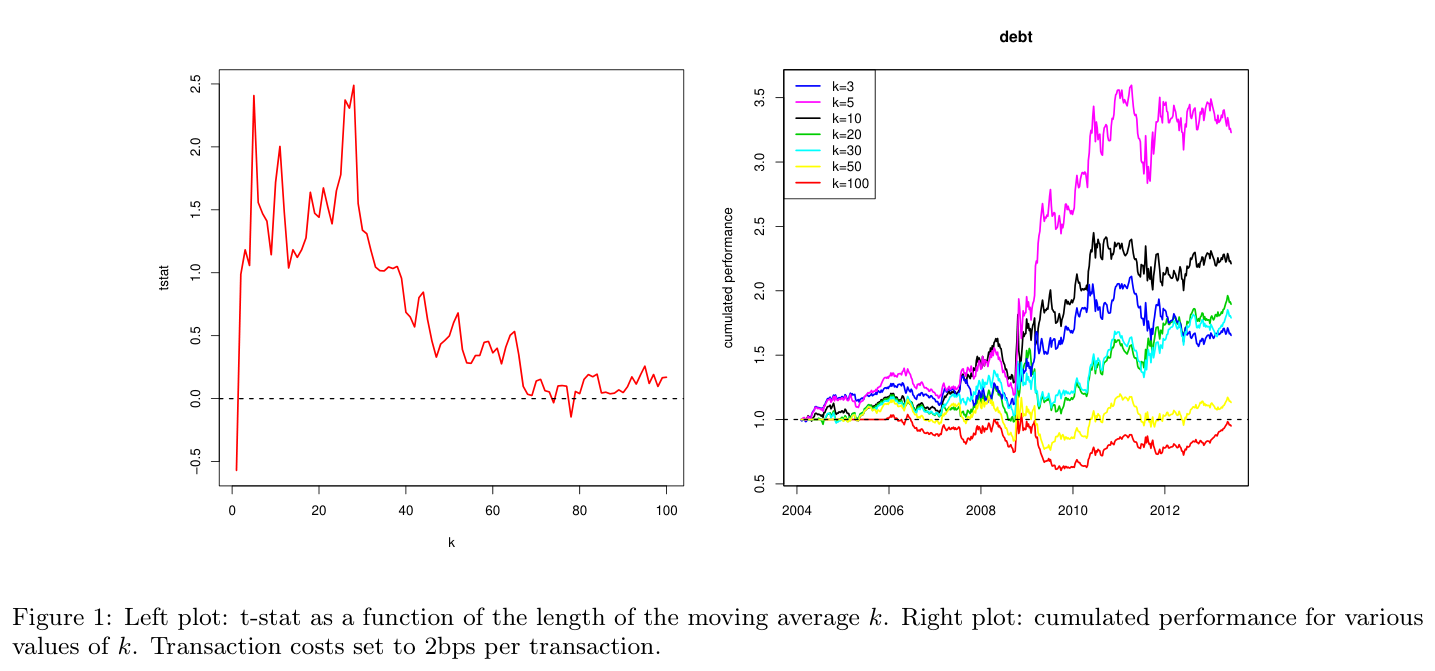
\includegraphics[width=0.8\linewidth]{gfx/m4l2_challetbel_fig1_tstat_vs_movwindow.png}
\par\smallskip{\small \textbf{Hình 1:} Đồ thị trái: t-stat theo hàm của độ dài cửa sổ trượt $k$. Đồ thị phải: hiệu suất tích lũy ứng với các giá trị khác nhau của $k$. Chi phí giao dịch được đặt ở mức 2bps mỗi lần giao dịch.}
\end{figure}

\begin{figure}[H]
\centering
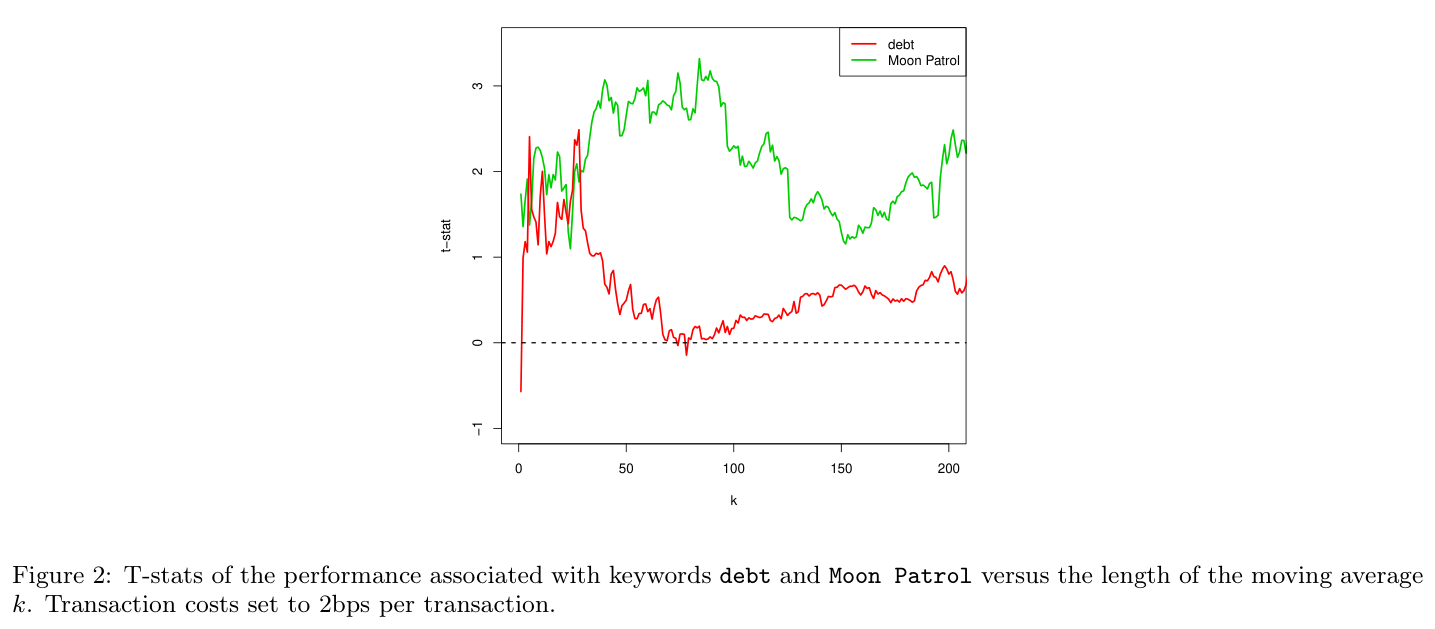
\includegraphics[width=0.8\linewidth]{gfx/m4l2_challetbel_fig2_tstat_debt_moonpatrol.png}
\par\smallskip{\small \textbf{Hình 2:} T-stat của hiệu suất gắn với các từ khóa \texttt{debt} và \texttt{Moon Patrol} theo độ dài của cửa sổ trượt $k$. Chi phí giao dịch được đặt ở mức 2bps mỗi lần giao dịch.}
\end{figure}

\section{IV. Sức Mạnh Dự đoán của Google Trends}

Với nhiều điểm yếu về phương pháp luận đã liệt kê ở trên, người ta có thể bắt đầu nghi ngờ các kết luận của [24]. Ở đây chúng tôi cho thấy rằng các kết luận đó là đúng. Bước đầu tiên là tránh những vấn đề phương pháp luận đã nêu ở trên. Một trong hai tác giả đã dùng một hệ thống backtest đạt chuẩn công nghiệp cùng các chiến lược tinh vi hơn (điều này do đó gây ra sai lệch công cụ). Trước tiên, hãy so sánh hiệu suất tích lũy thu được của ba tập từ khóa ngẫu nhiên mà chúng tôi đã định nghĩa, cộng với tập từ khóa lấy từ \emph{Financial Times}. Đối với mỗi tập từ khóa, chúng tôi chọn làm đầu vào: SVI thô, SVI trễ (lagged), và các đường trung bình trượt khác nhau của SVI, cùng với lợi suất chỉ số trong quá khứ. Kết quả cho thấy không có tập từ khóa nào mang lại thông tin có khả năng dự đoán đáng kể các biến động chỉ số (xem Hình 4). Điều này không mâu thuẫn với kết quả của [9, 11, 24]. Nó chỉ đơn giản có nghĩa là tín hiệu có lẽ quá yếu để có thể khai thác được trong thực tế. Phần cuối của các đường hiệu suất tất nhiên trông hấp dẫn, nhưng điều này xuất phát từ việc lợi suất SPY từ giá đóng cửa thứ Hai đến giá đóng cửa thứ Sáu phần lớn là dương trong giai đoạn này: bất kỳ thuật toán học máy nào chỉ áp dụng trên lợi suất cũng có khả năng cho ra kết quả tương tự.

\begin{figure}[H]
\centering
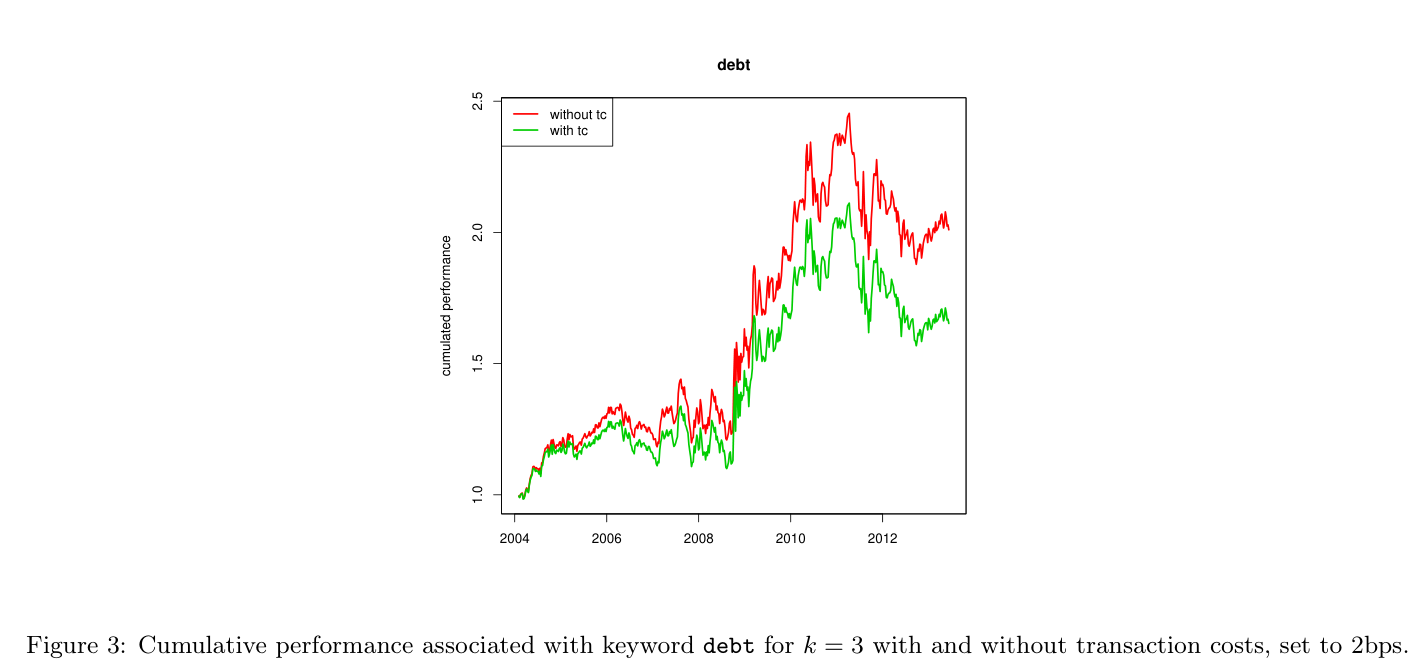
\includegraphics[width=0.6\linewidth]{gfx/m4l2_challetbel_fig3_cumperf_debt_tc.png}
\par\smallskip{\small \textbf{Hình 3:} Hiệu suất tích lũy gắn với từ khóa \texttt{debt} với $k=3$, có và không có chi phí giao dịch, được đặt ở mức 2bps.}
\end{figure}

\begin{figure}[H]
\centering
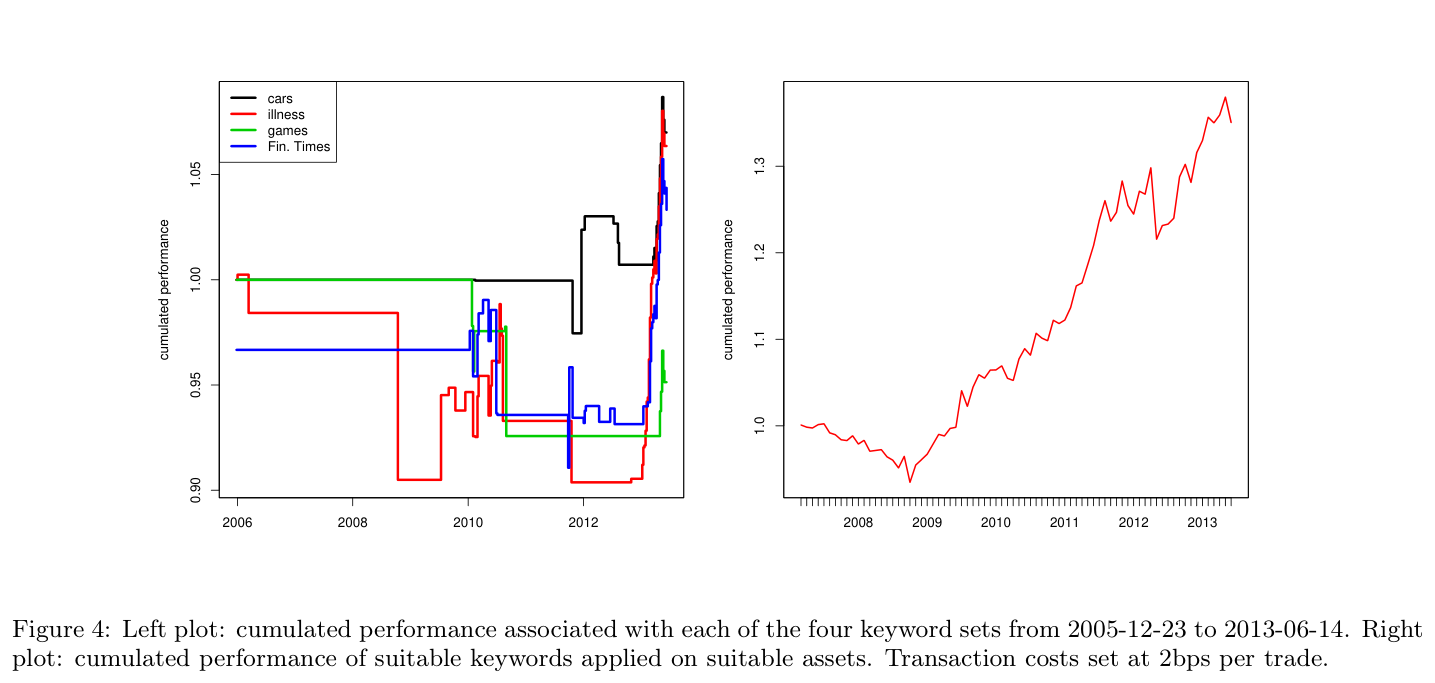
\includegraphics[width=0.8\linewidth]{gfx/m4l2_challetbel_fig4_cumperf_keyword_sets.png}
\par\smallskip{\small \textbf{Hình 4:} Đồ thị trái: hiệu suất tích lũy gắn với từng tập trong bốn tập từ khóa, từ 23/12/2005 đến 14/06/2013. Đồ thị phải: hiệu suất tích lũy của các từ khóa phù hợp áp dụng lên các tài sản phù hợp. Chi phí giao dịch được đặt ở mức 2bps mỗi giao dịch.}
\end{figure}

Cho đến nay, chúng tôi chỉ có thể kết luận rằng một hệ thống backtest đúng đắn (và không quá khắt khe) đã không thể tìm thấy bất kỳ thông tin nào có thể khai thác được từ bốn tập từ khóa, chứ không phải là các tập từ khóa đó không chứa đủ thông tin dự đoán. Để kết luận, chúng tôi sử dụng cùng hệ thống backtest với một số dữ liệu GT, dùng chính xác cùng các tham số và loại đầu vào như trước. Hiệu suất sơ bộ, báo cáo trong Hình 4, hứa hẹn hơn và cho thấy dữ liệu GT thực sự luôn chứa một lượng thông tin dự đoán nhất định. Hiệu suất này không đặc biệt ấn tượng khi so với hiệu suất của chính SPY, nhưng vẫn thú vị vì mức độ tiếp xúc ròng (net exposure) luôn gần bằng 0 (xem [6] để biết thêm thông tin).

\section{V. Thảo luận}

Cần có các phương pháp tinh vi kết hợp với backtest cẩn trọng để chứng minh rằng Google Trends chứa đủ thông tin có thể khai thác được. Điều này là do loại dữ liệu như vậy bao gồm quá nhiều lượt tìm kiếm có lẽ không liên quan đến tài sản tài chính ứng với một từ khóa cho trước, và thậm chí còn ít liên quan hơn nữa đến hoạt động giao dịch thực tế. Khi người ta thu hẹp phạm vi tìm kiếm bằng cách cung cấp nhiều từ khóa hơn, dữ liệu GT thường chỉ chứa thông tin ở quy mô thời gian hàng tháng, hoặc không chứa thông tin nào cả.

Nếu quay lại thuật toán được đề xuất bởi [24] và các phát hiện tương thích của [9, 11], thật khó để hiểu tại sao giá tương lai lại có xu hướng đảo chiều một cách hệ thống sau một bất ngờ SVI dương, và ngược lại một tuần sau đó. Hiện tượng đảo chiều này yếu và chỉ đúng tính trung bình. Đây có thể là kết quả phổ biến nhất, nhưng khả năng sinh lời sẽ cao hơn nhiều nếu người ta biết được điều gì kích hoạt sự đảo chiều hay sự tiếp diễn xu hướng (trend following). Có một số bằng chứng cho thấy việc bổ sung dữ liệu GT bằng tin tức dẫn đến hiệu suất giao dịch được cải thiện đáng kể (xem ví dụ [4]).

Một bài báo khác của cùng nhóm tác giả đề xuất một nguồn thông tin hứa hẹn hơn nhiều: bài báo đó liên hệ những thay đổi trong số lượt truy cập các trang Wikipedia của các công ty cho trước với lợi suất chỉ số trong tương lai [22]. Các nghiên cứu tiếp theo sẽ tìm hiểu sức mạnh dự đoán của loại dữ liệu này.

\section*{Lời cảm ơn}

Chúng tôi xin ghi nhận những cuộc trao đổi hữu ích với Frédéric Abergel, Marouanne Anane và Thierry Bochud.

% [Đã lược bỏ danh mục Tài liệu tham khảo gốc (tiếng Anh, trích dẫn của tác giả bài gốc) để giảm dung lượng chương; không ảnh hưởng nội dung học thuật chính.]

\section*{Phụ lục A: Từ khóa}

Chúng tôi đã tải xuống dữ liệu GT cho các từ khóa sau đây, không qua bất kỳ chỉnh sửa thủ công nào. (Các danh sách từ khóa dưới đây được giữ nguyên bằng tiếng Anh vì đây là các cụm tìm kiếm chính xác đã được dùng để truy vấn Google Trends; việc dịch sang tiếng Việt sẽ làm thay đổi từ khóa thực tế được sử dụng trong bài báo.)

\subsection*{1. Bệnh tật (Illnesses)}

\noindent Nguồn: \url{http://www.ranker.com/list/list-of-common-diseases-most-common-illnesses/diseases-and-medications-info}, truy cập ngày 27 tháng 5 năm 2013.

\smallskip
\noindent\small AIDS, Acne, Acute bronchitis, Allergy, Alopecia, Altitude sickness, Alzheimer's disease, Andropause, Anorexia nervosa, Antisocial personality disorder, Arthritis, Asperger syndrome, Asthma, Attention deficit hyperactivity disorder, Autism, Avoidant personality disorder, Back pain, Bad Breath, Bedwetting, Benign prostatic hyperplasia, Bipolar disorder, Bladder cancer, Bleeding, Body dysmorphic disorder, Bone cancer, Borderline personality disorder, Bovine spongiform encephalopathy, Brain Cancer, Brain tumor, Breast cancer, Burns, Bursitis, Cancer, Canker Sores, Carpal tunnel syndrome, Cervical cancer, Cholesterol, Chronic Childhood Arthritis, Chronic Obstructive Pulmonary Disease, Coeliac disease, Colorectal cancer, Conjunctivitis, Cradle cap, Crohn's disease, Dandruff, Deep vein thrombosis, Dehydration, Dependent personality disorder, Depression, Diabetes mellitus, Diabetes mellitus type 1, Diaper rash, Diarrhea, Disabilities, Dissociative identity disorder, Diverticulitis, Down syndrome, Drug abuse, Dysfunctional uterine bleeding, Dyslexia, Ear Infections, Ear Problems, Eating Disorders, Eczema, Edwards syndrome, Endometriosis, Epilepsy, Erectile dysfunction, Eye Problems, Fibromyalgia, Flu, Fracture, Freckle, Gallbladder Diseases, Gallstone, Gastroesophageal reflux disease, Generalized Anxiety Disorder, Genital wart, Glomerulonephritis, Gonorrhoea, Gout, Gum Diseases, Gynecomastia, HIV, Head Lice, Headache, Hearing impairment, Heart Disease, Heart failure, Heartburn, Heat Stroke, Heel Pain, Hemorrhoid, Hepatitis, Herniated Discs, Herpes simplex, Hiatus hernia, Histrionic personality disorder, Hyperglycemia, Hyperkalemia, Hypertension, Hyperthyroidism, Hypothyroidism, Infectious Diseases, Infectious mononucleosis, Infertility, Influenza, Iron deficiency anemia, Irritable Male Syndrome, Irritable bowel syndrome, Itching, Joint Pain, Juvenile Diabetes, Kidney Disease, Kidney stone, Leukemia, Liver tumour, Lung cancer, Malaria, Melena, Memory Loss, Menopause, Mesothelioma, Migraine, Miscarriage, Mucus In Stool, Multiple sclerosis, Muscle Cramps, Muscle Fatigue, Muscle Pain, Myocardial infarction, Nail Biting, Narcissistic personality disorder, Neck Pain, Obesity, Obsessive-compulsive disorder, Osteoarthritis, Osteomyelitis, Osteoporosis, Ovarian cancer, Pain, Panic attack, Paranoid personality disorder, Parkinson's disease, Penis Enlargement, Peptic ulcer, Peripheral artery occlusive disease, Personality disorder, Pervasive developmental disorder, Peyronie's disease, Phobia, Pneumonia, Poliomyelitis, Polycystic ovary syndrome, Post-nasal drip, Post-traumatic stress disorder, Premature birth, Premenstrual syndrome, Propecia, Prostate cancer, Psoriasis, Reactive attachment disorder, Renal failure, Restless legs syndrome, Rheumatic fever, Rheumatoid arthritis, Rosacea, Rotator Cuff, Scabies, Scars, Schizoid personality disorder, Schizophrenia, Sciatica, Severe acute respiratory syndrome, Sexually transmitted disease, Sinusitis, Skin Eruptions, Skin cancer, Sleep disorder, Smallpox, Snoring, Social anxiety disorder, Staph infection, Stomach cancer, Strep throat, Sudden infant death syndrome, Sunburn, Syphilis, Systemic lupus erythematosus, Tennis elbow, Termination Of Pregnancy, Testicular cancer, Tinea, Tooth Decay, Traumatic brain injury, Tuberculosis, Ulcers, Urinary tract infection, Urticaria, Varicose veins.
\normalsize

\subsection*{2. Xe cổ (Classic cars)}

\noindent Nguồn: \url{http://www.ranker.com/crowdranked-list/the-best-1960_s-cars}, truy cập ngày 27 tháng 5 năm 2013.

\smallskip
\noindent\small 1960 Aston Martin DB4 Zagato, 1960 Ford, 1961 Ferrari 250 SWB, 1961 Ferrari 250GT California, 1963 Corvette, 1963 Iso Griffo A3L, 1964 Ferrari 250 GTL (Lusso), 1965 Bizzarrini 5300 Strada, 1965 Ford GT40, 1965 Maserati Mistral, 1965 Shelby Cobra, 1966 Ferrari 365P, 1966 Maserati Ghibli, 1967 Alfa Romeo Stradale, 1967 Ferrari 275 GTB/4, 1967 Shelby Mustang KR500, 1968 Chevrolet Corvette L88, 1968 DeTomaso Mangusta, 1969 Pontiac Trans Am, 1969 Yenko Chevelle, 57 Chevy, 68 Ferrari 365 GTB/4 Daytona Spyder, 69 Yenko Camaro Z28, AC Cobra, Alfa Romeo Spider, Aston Martin DB5, Austin Mini Saloon 1959, BMW E9, Buick Riviera, Buick Wildcat, Cane, Chevrolet Camaro, Chevrolet Chevelle, Chevrolet Impala, Chevy Chevelle, Chrysler Valiant, Corvette Stingray, Dodge Challenger, Dodge Charger, Dodge Dart Swinger, Facel Vega Facel II, Ferrari 250, Ferrari 250 GTO, Ferrari 275, Ferrari Daytona, Fiat 500, Ford Corsair, Ford Cortina, Ford GT40, Ford Mustang, Ford Ranchero, Ford Thunderbird, Ford Torino, Ford Zephyr MK III, Iso Grifo, Jaguar E-type, Jeep CJ, Lamborghini Miura, Lamborghini Miura SV, Lincoln Continental, Lotus Elan, Maserati Ghibli, Mercedes Benz 220SE, Mercedes-Benz 300SL, Mercury Cougar, Plymouth Barracuda, Pontiac GTO, Porsche 356, Porsche 911, Porsche 911 classic, Shelby GT500, Rambler Classic, Rover 2000, Shelby Daytona Coupe, Shelby GT350, Studebaker Avanti, Sunbeam Tiger, Toyota 2000GT, Triumph 2000, Vauxhall Velox 1960, Vauxhall Victor 1963, Wolseley 15/60.
\normalsize

\subsection*{3. Trò chơi thùng (Arcade Games)}

\noindent Nguồn: \url{http://www.ranker.com/list/list-of-common-diseases-most-common-illnesses/diseases-and-medications-info}, truy cập ngày 27 tháng 5 năm 2013. (Ghi chú của người dịch: đây là URL nguồn được ghi trong bản gốc của bài báo cho danh sách này; có khả năng là một sơ suất trong tài liệu gốc, được giữ nguyên theo đúng bản gốc để không làm sai lệch nội dung.)

\smallskip
\noindent\small 1942, 1943, 720\textdegree{}, After Burner, Airwolf, Altered Beast, Arkanoid, Asteroids, Bad Dudes Vs. DragonNinja, Bagman, Battlezone, Beamrider, Berzerk, Bionic Commando, Bomb Jack, Breakout, Bubble Bobble, Bubbles, BurgerTime, Centipede, Circus Charlie, Commando, Crystal Castles, Cyberball, Dangar - Ufo Robo, Defender, Dig Dug, Donkey Kong, Donkey Kong 3, Donkey Kong Junior, Double Dragon, Dragon's Lair, E.T. (Atari 2600), Elevator Action, Final Fight, Flashback, Food Fight, Frogger, Front Line, Galaga, Galaxian, Gauntlet, Geometry Wars, Gorf, Gyruss, Hogan's Alley, Ikari Warriors, Joust, Kangaroo, Karate Champ, Kid Icarus, Lode Runner, Lunar Lander, Manic Miner, Mappy, Marble Madness, Mario Bros., Millipede, Miner 2049er, Missile Command, Moon Buggy, Moon Patrol, Ms. Pac-Man, Naughty Boy, Pac-Man, Paperboy, Pengo, Pitfall!, Pole Position, Pong, Popeye, Punch-Out!!, Q*bert, Rampage, Red Baron, Robotron: 2084, Rygar: The Legendary Adventure, Sewer Sam, Snow Bros, Space Invaders, Spy Hunter, Star Wars, Stargate, Street Fighter, Super Pac-Man, Tempest, Tetris, The Adventures of Robby Roto!, The Simpsons, Time Pilot, ToeJam \& Earl, Toki, Track \& Field, Tron, Wizard Of Wor, Xevious.
\normalsize

\section*{Phụ lục B: Mã nguồn}

Dưới đây là một cách hiện thực đơn giản bằng ngôn ngữ R cho chiến lược được trình bày trong [24]. Chúng tôi dùng ký hiệu ``='' thay vì ``<-'' để gán giá trị.

\begin{verbatim}
computePerfStats=function(filename,k=10,getPerf=FALSE){
        gtdata=loadGTdata(filename)
        if(is.null(gtdata) || length(gtdata)<100){
                return(NULL)
        }
        spy=loadYahooData('SPY')
        spy_rets=getFutureReturns(spy)        #spy_rets is a zoo object, contains r_{t+1}
        gtdata_mean=rollmeanr(gtdata,k)        # \bar v_t
        gtdata_mean_lagged=lag(gtdata_mean,-1) # \bar v_{t-1}
        pos=2*(gtdata>gtdata_mean_lagged)-1
        perf=-pos*spy_rets
        perf=perf[which(!is.na(perf))]
        if(getPerf){
                return(perf)
        }else{
                return(t.test(perf)$statistic)
        }
}
\end{verbatim}

